\documentclass{article}
\usepackage[main=spanish, provide=*]{babel}
\usepackage{xcolor}
\usepackage{array}
\usepackage{graphicx}
\usepackage{tikz}
\usepackage{circuitikz}
\usepackage{pgfplots}
\usepackage{darkmode}
\usepackage{amsmath}
\usepackage[a4paper, top=2cm, bottom=2cm]{geometry}
\usepackage{chngcntr}
\counterwithin{figure}{section}
\usepackage{caption}

% Redefinir el formato de las figuras
\captionsetup[figure]{labelsep=none}



\enabledarkmode

\definecolor{c1}{HTML}{8bb6e7}
\definecolor{c2}{HTML}{87f3dd}
\definecolor{c3}{HTML}{fdef83}
\definecolor{c4}{HTML}{fdc373}
\definecolor{c5}{HTML}{fd8581}
\definecolor{c6}{HTML}{c573e7}
\definecolor{c7}{HTML}{afdb68}
\definecolor{c8}{HTML}{e59f8b}

\definecolor{page}{HTML}{262626}
\pagecolor{page}

\begin{document}
\title{EXAMEN RECUP 1 (TEMAS 1 al 4)}
\author{Mario López Sáez}
\date{\today}
\maketitle

\begin{center}

\begin{tikzpicture}
    \fill[c1] (0, 0) rectangle ++(1, 0.05);
    \fill[c2] (1, 0) rectangle ++(1, 0.05);
    \fill[c3] (2, 0) rectangle ++(1, 0.05);
    \fill[c4] (3, 0) rectangle ++(1, 0.05);
    \fill[c5] (4, 0) rectangle ++(1, 0.05);
    \fill[c6] (5, 0) rectangle ++(1, 0.05);
    \fill[c7] (6, 0) rectangle ++(1, 0.05);
    \fill[c8] (7, 0) rectangle ++(1, 0.05);
\end{tikzpicture}

\end{center}

\section{CUESTIÓN (2.5 p)}
\begin{center}
    
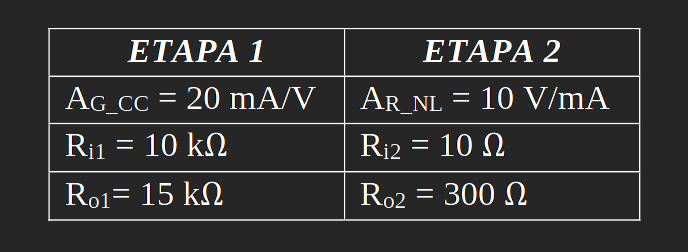
\includegraphics[width=0.5\textwidth]{tabla1.jpg} 
\end{center}



\begin{figure}[h!]
    \centering
    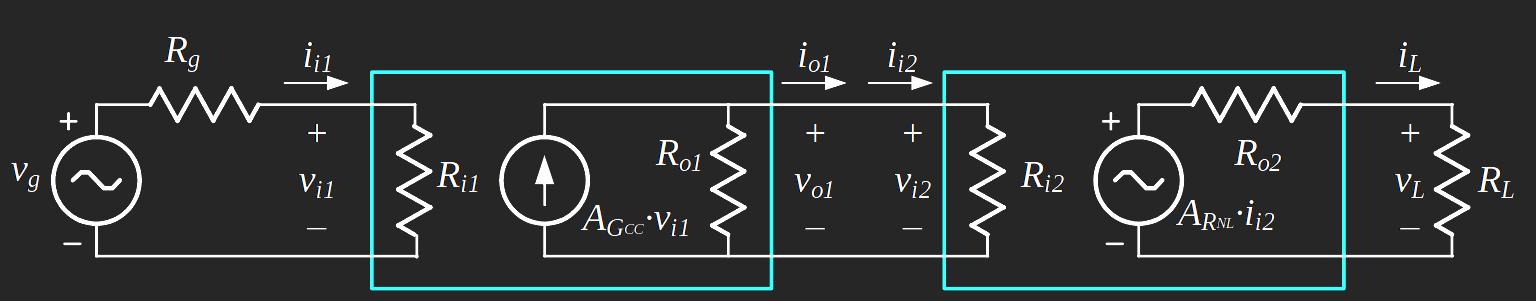
\includegraphics[width=0.7\textwidth]{fig11.jpg} 
    \caption{}
\end{figure}

\begin{figure}[h!]
    \centering
    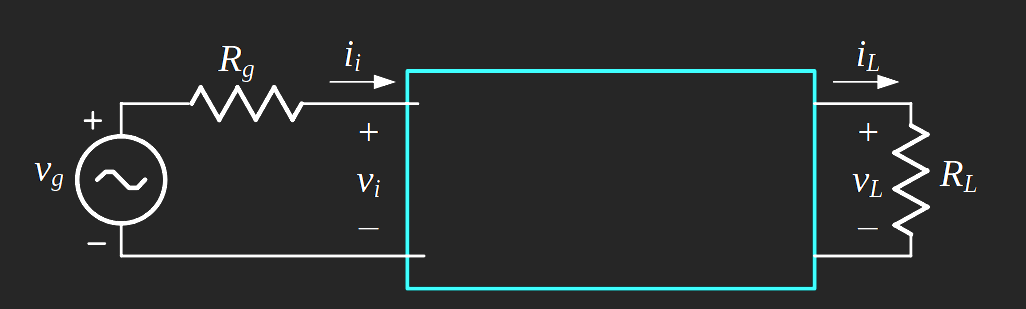
\includegraphics[width=0.5\textwidth]{fig12.jpg} 
    \caption{}
\end{figure}

\begin{flushleft}
Disponemos de los modelos de dos etapas amplificadoras conectadas en cascada según
se indica en la figura 1.1. Obtener el modelo equivalente del amplificador de TENSIÓN resultante de la combinación de ambas etapas: \newline

    
\textbf{a) (0.5 p.) Dibujar} el modelo de TENSIÓN resultante en la Figura 1.2 \\
\textbf{b) (1.5 p.) Calcular} el valor de sus parámetros del amplificador de TENSIÓN resultante, a partir de los valores de las etapas que lo componen.
$$
i_{i2} = A_{G_{CC}} \cdot V_{i1} \cdot \frac{R_{o1}}{R_{o1} + R_{i2}}
$$

$$
\frac{R_{o1}}{R_{o1} + R_{i2}} = \frac{15 \text{k} \Omega}{15 \text{k} \Omega + 10 \Omega} = 0.9993
$$

$$
i_{i2} \approx A_{G_{CC}} \cdot V_{i1}
$$


\end{flushleft}

\begin{center}
	\begin{circuitikz}[american]
		\draw (0, 0) to[vsourcesin, v^<=$V_g$] (0, 2) to[R = $R_g$] (2, 2);
		\draw (0, 0) to[short] (2, 0);
		\draw (2, 2) to[short] (3, 2) to[R=$R_{i1}$] (3, 0) to[short] (2, 0);
		\draw (2, 2) to[open, v=$V_i$] (2, 0);
		\draw (6, 0) to[vsourcesin, v_<=$200 \cdot V_{i1}$] (6, 2) to[R = $R_{o2}$, i=$i_L$] (10, 2) to[R = $R_L$, v_=$V_L$] (10, 0) to[short] (6, 0);
		\draw[c2, thick] (2.5, 2.25) -- (2.5, -0.25) -- (8.7, -0.25) -- (8.7, 2.25) -- (2.5, 2.25);
    \end{circuitikz}
\end{center}

\subsection{Solución formal}
\paragraph{Impedancia de entrada}
$$
R_{i}=\frac{v_{i}}{i_{i}}=\frac{v_{i1}}{i_{i1}}=R_{i}=\,10\,\mathrm{k} \Omega = R_{i1}
$$

\paragraph{Ganancia de tensión sin carga}
$$
A_{vN L}=\frac{v_{o N L}}{v_{i}}=A_{RN L}\cdot\,A_{G_{CC}}\cdot\frac{R_{o1}}{R_{o1}+R_{i2}}=199.87\simeq200\,V/V
$$

\paragraph{Impedancia de salida}
\begin{center}
    
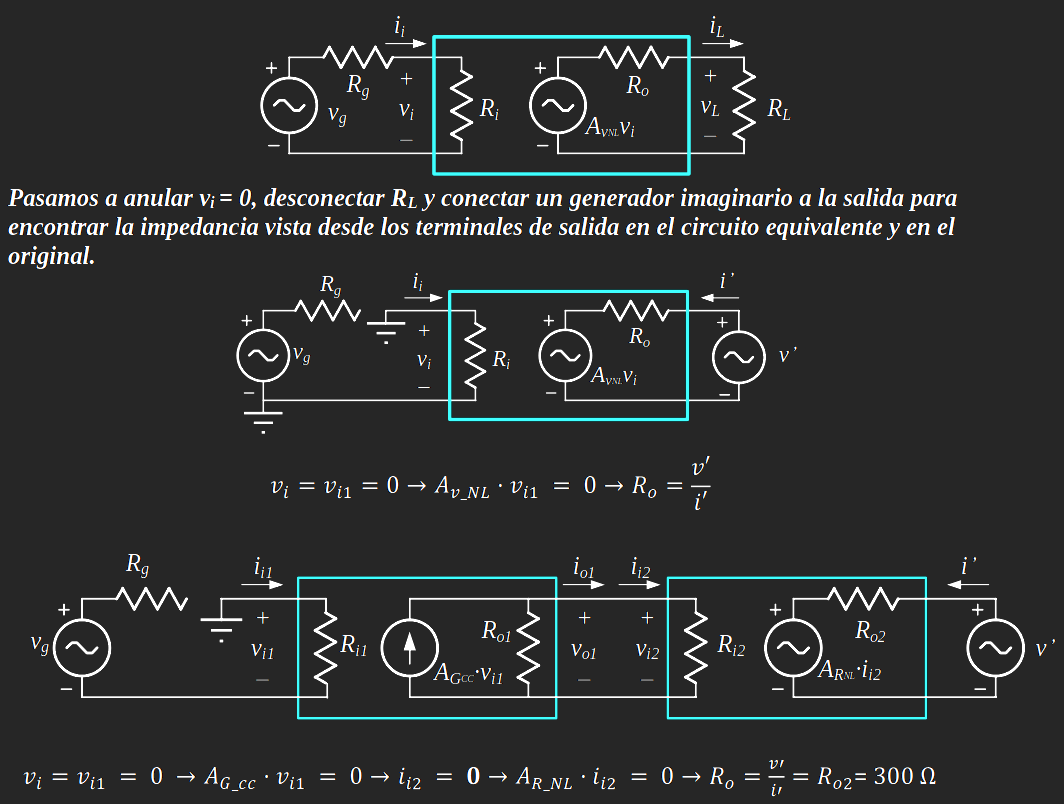
\includegraphics[width=\textwidth]{pagcop1.jpg} 
\end{center}


\begin{center}
	\begin{circuitikz}[american]
		\draw (0, 0) to[vsourcesin, v^<=$V_g$] (0, 2) to[R = $R_g$] (2, 2);
		\draw (0, 0) to[short] (2, 0);
		\draw (2, 2) to[short] (3, 2) to[R=$R_{i}$] (3, 0) to[short] (2, 0);
		\draw (2, 2) to[open, v=$V_i$] (2, 0);
		\draw (6, 0) to[vsourcesin, v_<=$A_{\text{VNL}} \cdot V_{i}$] (6, 2) to[R = $R_{o}$, i=$i_L$] (10, 2) to[R = $R_L$, v_=$V_L$] (10, 0) to[short] (6, 0);
		\draw[c2, thick] (2.5, 2.25) -- (2.5, -0.25) -- (8.7, -0.25) -- (8.7, 2.25) -- (2.5, 2.25);
    \end{circuitikz}
\end{center}

\begin{flushleft}
\textbf{c) (0.5 p.) Calcular} el valor de tensión $v_L$ que aparecerá en bornes de $R_L = 10 k \Omega$, si a la entrada se conecta un generador $v_g = 100 mV_p$, y $R_g = 100 \Omega$ \\
$$
V_L = 200 \cdot 100 mV_p \cdot \frac{10 k \Omega}{10 k \Omega + 100 \Omega} \cdot \frac{10 k \Omega}{10 k \Omega + 300 \Omega} = 19.225 \ V_p
$$

\end{flushleft}

\section{CUESTIÓN (2.5 puntos)}
\begin{figure}[h!]
    \centering
    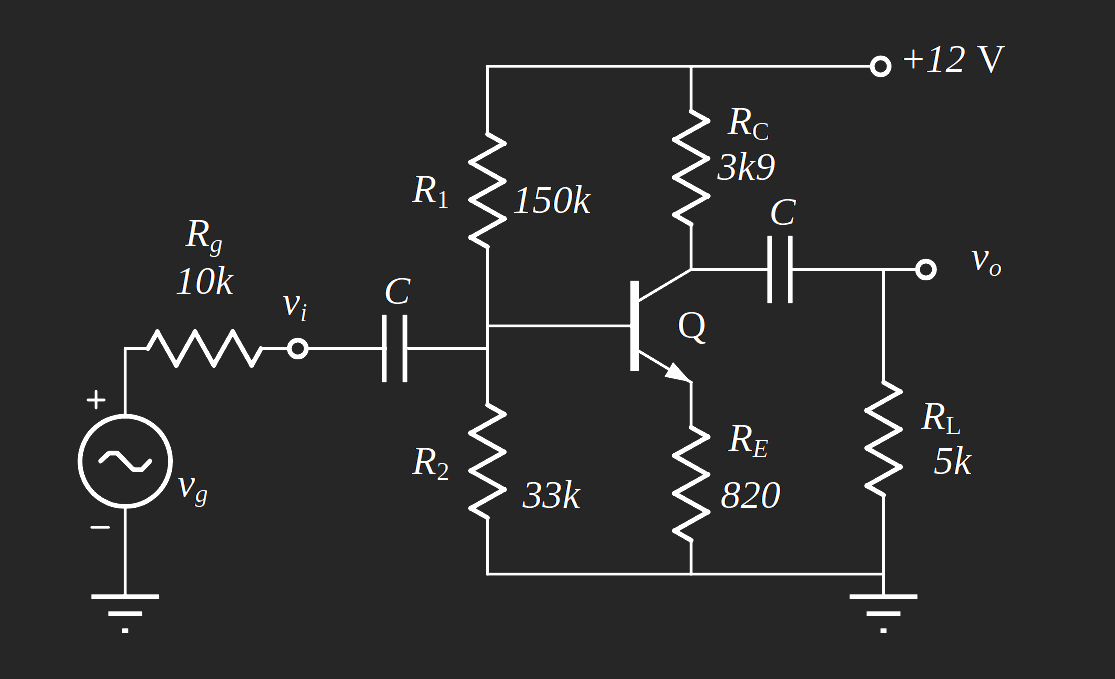
\includegraphics[width=0.5\textwidth]{fig2.jpg} 
    \caption{}
    \label{fig:ejemplo}
\end{figure}
\begin{flushleft}
\textbf{a) (0.5 p.)} Obtener su punto de trabajo \textbf{Q}
$$
V_{C C}=12 V;R_{C}=3,9{\mathrm{~k}}\Omega;R_{E}=0,82{\mathrm{~k}}\Omega;R_{1}=150{\mathrm{~k}}\Omega;R_{2}=33{\mathrm{~k}}\Omega;R_{L}=5{\mathrm{~k}}\Omega;C\rightarrow\infty
$$
$$
{\mathrm{Q~}}\{h_{f e}\simeq\beta=100; V_{B E}=O,7\mathrm{V};\,h_{o e}=0\}
$$



\end{flushleft}




\begin{center}
	\begin{circuitikz} 
		\draw (-1, 0) node[above] {$v_i$} to[short, o-] (0, 0) to[R=$150k$] (0, 4) to[short] (4, 4) to[short, -*] (6, 4) node[right] {$12V$}; 
		\draw (3, 0) node[npn, anchor=B](Q1) {Q1};
		\draw (0, 0) to[short] (Q1.B);
		\draw (Q1.C) to[R = $3k9$] (Q1.C |- 0,4);
		\draw (Q1.E) to[R, l_=$820$] (Q1.E |- 0,-4) to[short] (0, -4) to[R, l=$33k$] (0, 0);
		\draw (Q1.C) to[short, -*] (6,0 |- Q1.C) node[right] {$v_o$};
		\draw (2, -4) node[ground](){};
    \end{circuitikz}
\end{center}
$$
V_B = 12 \cdot \frac{33k}{150k+33k} = 2.16 V
$$
$$
R_{BB} = \frac{150k \cdot 33k}{183k} = 27.05 \ k \Omega
$$
$$
V_E = 2.16 - 0.7 = 1.46 V
$$
$$
I_E = \frac{V_E}{820} = 1.79 \ mA \approx I_C
$$
$$
v_o = 12 - I_C \cdot 3k9 = 5.04 V
$$

\begin{quote}
	\textcolor{c5!50!red}{Los resultados dados por los profesores varían ligeramente, y no he podido encontrar la razón. A partir de aquí se usarán los valores $I_C = 1.33 \text{ mA}$ y $V_{CE} =  5.7 \text{ V}$}
\end{quote}

\newpage

\begin{flushleft}
\textbf{b) (1.25 p.)} Obtener y dibujar la recta de carga dinámica
$$
i_{C}-I_{C_Q}=m_{d}\cdot(v_{C E}-V_{C E_{Q}})
$$
\end{flushleft}

\begin{center}
    \begin{circuitikz}[american]

	    \draw (0, 0) node[ground](){};
	    \draw (6, 2) node[npn, anchor=B](Q1) {Q1};
	    \draw (2, 0) node[ground](G1){};
	    \draw (4, 0) node[ground](G2){};
	    \draw (Q1.E |- 0, 0) node[ground](GE){};
	    \draw (0, 0) to[vsourcesin, v^<=$v_g$] ++(0, 2) to[R = $R_g$] ++(2, 0) to [R, l_=$150 \text{k}$] ++(0, -2);
	    \draw (4, 2) to [R, l_=$33 \text{k}$] ++(0, -2);
	    \draw (2, 2) to [short] ++(4, 0);
	    \draw[c1] (GE) to[R = $820$] (Q1.E);
	    \draw (Q1.C) to [short] ++(2, 0) coordinate(aux) to [R,color=c3, l_=$3k9$, c3] (aux |- G1) node[ground](){};
	    \draw (aux) to [short] ++(2, 0) coordinate(aux) to [R,color=c3, l_=$5k$,c3] (aux |- G1) node [ground] () {};
	    \draw (aux) to [short, -o] ++(1, 0) node [right] {$v_o$}; 

    \end{circuitikz}
\end{center}
$$
m_d = \frac{-1}{\textcolor{c1}{820}+ \textcolor{c3}{3k9 || 5k}} = -0.332 \text{ mA/V}
$$
$$
i_C - 1.33 = -0.332 \cdot (v_{CE} - 5.7)
$$
$$
i_C = -0.332 v_{CE} + 3.225
$$

\begin{center}
    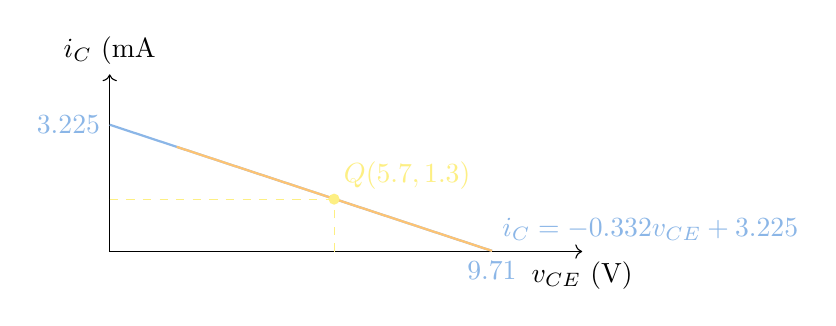
\begin{tikzpicture}
	    \draw [->] (0, 0) -- ++(12/2, 0) node [below] {$v_{CE} \text{ (V)}$} ;
    \draw [->] (0, 0) -- ++(0, 2.25) node [above] {$i_C \text{ (mA}$} ;
        \draw[thick, c1, domain=0:9.71/2] 
            plot (\x, {-0.33*\x + 3.22/2}) 
            node[above right] {$i_C = -0.332 v_{CE} + 3.225$}
	    node[below] {$9.71$};
    \draw[c1] (0,3.225/2) node[left] {$3.225$};
    \draw[c3, dashed] (5.7/2, 0) -- (5.7/2, 1.33/2);
    \draw[c3, dashed] (0, 1.33/2) -- (5.7/2, 1.33/2) coordinate(Q);
    \draw[thick, c4, domain=1.7/2:9.71/2] 
            plot (\x, {-0.33*\x + 3.22/2}); 

    \fill[c3] (Q) circle (2 pt) node [above right] {$Q (5.7, 1.3)$} ;
    \end{tikzpicture}
\end{center}
$$
\color{c4}{\Delta i_c \text{ simétrica máx} = \pm 1.33 \text{ mA}}
$$

\begin{flushleft}
\textbf{c) (0.75 p.) }A partir de la recta de carga dinámica, calcular la máxima excursión simétrica de la señal
de salida ($\Delta v_L$ máximo) del amplificador, en voltios de pico a pico.
\end{flushleft}
$$
i_C \text{ máx} = 2.6 \text{ mA}
$$
$$
v_o = v_L = v_{R_C} \to v_L \text{máx} = 2.6 \cdot \textcolor{c3}{3.9||5} = 5.83 \text{ V}_{pp}
$$

\section{CUESTIÓN (2.5 p.)}
\paragraph{\textbf{DATOS: } $V_{D D}=+5 \text{ V};-V_{S S}=-5 \text{ V};R_{G}=22~\mathrm{k} \Omega;~C\to\infty$ \newline} 
MOSFET: {$K = 5 \text{mA/V}^2 ; \ V_T = 4 \text{ V} ; r_d \to \infty$}
\begin{figure}[h!]
    \centering
    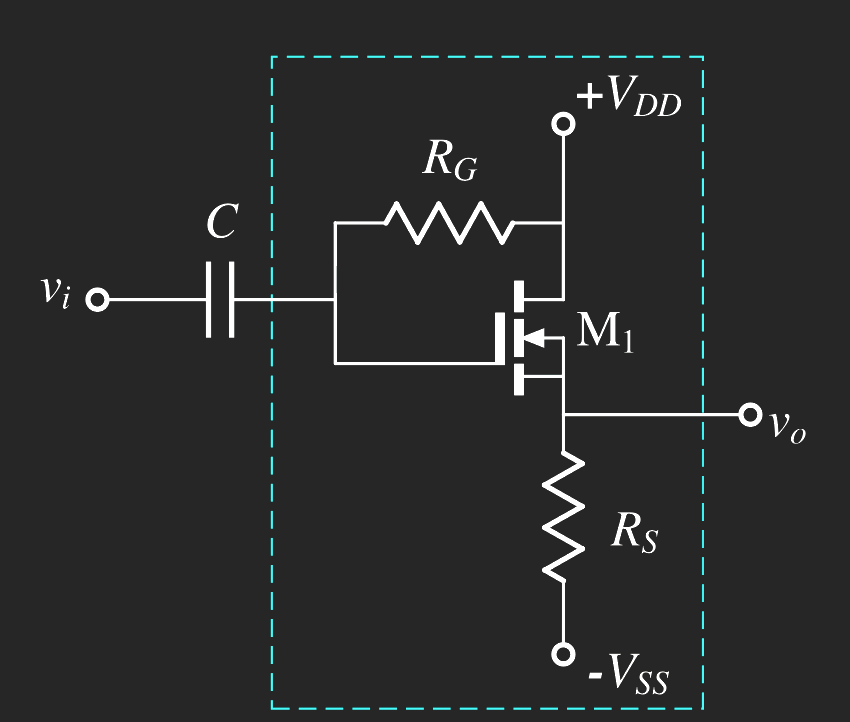
\includegraphics[width=0.5\textwidth]{fig3a.jpg} 
    \caption{}
\end{figure}

\begin{flushleft}
\textbf{a) (0.5 p.)} Calcular el valor de la resistencia $R_S$ necesario para que en el punto de reposo ($v_i = 0$) la tensión en DC (continua) en la salida $v_o$, es decir en la fuente o surtidor de M1 corresponda con 0 V (VS = 0).
Obtener el modelo y el valor del parámetro gm para el mosfet M1 en pequeña señal (AC).
\end{flushleft}

$$
I_{G} = 0; \ V_{G} = +V_{DD} = 5 \text{ V}
$$
$$
V_{S} = 0 \text{ V}
$$
$$
V_{GS} = 5 \text{ V}
$$

\textbf{Suponemos región activa }$\to I_{D} \approx K(V_{GS} - V_{T})^{\textcolor{c1}{2}} = 5 \text{ mA}$

\textbf{Cálculo de $g_{m}$}
$$
g_{m} = \frac{\partial i_{d} }{\partial v_{gs}} = \textcolor{c1}{2} K (v_{GS} - V_{T}) \approx 2K(V_{GS_Q} - V_{T}) = 10 \ \frac{\text{mA}}{\text{V}}
$$

\textbf{RS} necesaria
$$
V_{o} = I_{D} \cdot R_{S} - 5
$$
$$
0 = 5 \text{ mA} \cdot R_{S} - 5 \text{ V}
$$
$$
R_{S} = 1 \text{ k} \Omega
$$

\begin{center}
    \begin{tikzpicture}
        \draw (0, 0) -- (0.9\textwidth, 0);
    \end{tikzpicture}
\end{center}

\begin{figure}[h!]
    \centering
    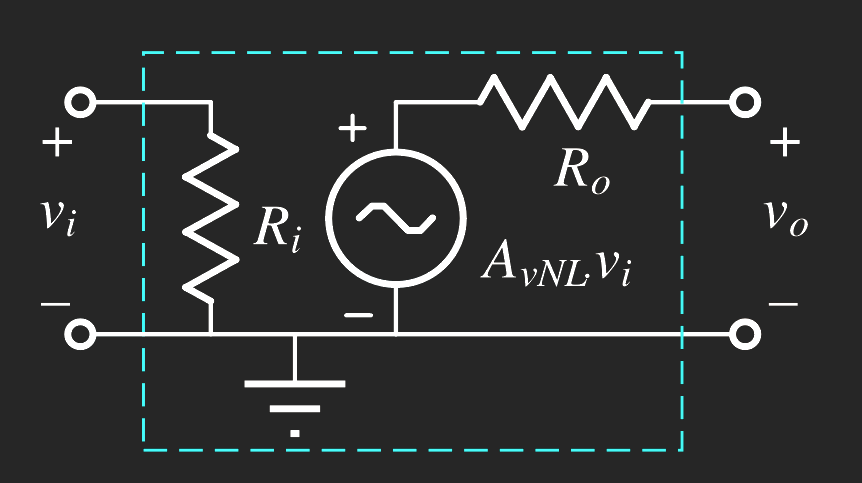
\includegraphics[width=0.5\textwidth]{fig32.jpg} 
    \caption{}
\end{figure}
\begin{flushleft}
    
\textbf{b) (1 p.)} Dibuja el modelo en pequeña señal del circuito para frecuencias medias y obtener justificadamente el valor de los parámetros del modelo equivalente del amplificador de tensión correspondiente de acuerdo con esquema de la figura 3.2: la ganancia en vacío AvNL y las resistencias de entrada y salida $R_{i}$ y $R_{o}$
\end{flushleft}

\begin{center}
    \begin{circuitikz}[american]
        \draw (0,-3) node [ground] () {} to [vsourcesin, l=$v_{g}$] ++(0, 5)
	to [R, l=$R_{g}$] ++(2, 0) to[short, color=c1, -*] ++(0.5,0) coordinate(vi) to [short] ++(1,0) coordinate(G1) to [R, l=$R_{G}$] ++(0, -3) coordinate(aux);
	\draw (aux |- 0, -3) node[ground](){} to [short] ++(0, 2);
	\draw (G1) to[short, i=0, c5!50!red, -*] ++(1.5,0) coordinate(G) node[above] {G};
	\draw (G |- 0,-1) coordinate(S) node[above] {S} to[short, *-] ++(2, 0) coordinate(RS) to [R, l=$R_{S}$] ++(0, -3) coordinate(aux);
	\draw (aux) node[ground](){} to [short, color=c1, -*] (vi |- aux) to[open, v<=$v_{i}$, c1, color=c1] (vi);
	\draw (G) to[open, v=$v_{GS}$] (S);
	\draw (RS) to[short] ++(2,0) coordinate(ISO);
	\draw (RS) to[open] ++(0,-0.5) to [short, -*] ++(3,0) node [right] {$v_{o}$};
	\draw (ISO |- 0,2) coordinate(aux) to[isource, l=$g_{m}v_{GS}$] ++(0, -3);
	\draw (aux) to [short, -*] ++(2,0) node[above] {D} node[ground](){};


    \end{circuitikz}
\end{center}
\newpage
\textbf{IMPEDANCIA DE SALIDA}
\begin{center}
    \begin{circuitikz}[american]
        \draw (0,-3) node [ground] () {} to [vsourcesin, l=$v_{g}$] ++(0, 5)
	to [R, l=$R_{g}$] ++(2, 0) to[open] ++(0.5,0) coordinate(vi) to [short] ++(1,0) coordinate(G1) to [R, l=$R_{G}$] ++(0, -3) coordinate(aux);
	\draw (aux |- 0, -3) node[ground](){} to [short] ++(0, 2);
	\draw (G1) to[short, i=0, c5!50!red, -*] ++(1.5,0) coordinate(G) node[above] {G};
	\draw (G |- 0,-1) coordinate(S) node[above] {S} to[short, *-] ++(2, 0) coordinate(RS) to [R, l=$R_{S}$] ++(0, -3) coordinate(aux);
	\draw (aux) node[ground](){} to [short, color=c3, -*] (vi |- aux) to[open, v<=$0$, c3, color=c3] (vi);
	\draw [c3] (vi) node[ground](){};
	\draw (G) to[open, v=$v_{GS}$] (S);
	\draw (RS) to[short] ++(2,0) coordinate(ISO);
	\draw [c3] (RS) to[open] ++(0,-0.5) to [short, -*] ++(3,0) to[vsourcesin, l=$v'$, i=$i'$] ++(0, -2.5) node [ground](){};
	\draw (ISO |- 0,2) coordinate(aux) to[isource, l=$g_{m}v_{GS}$] ++(0, -3);
	\draw (aux) to [short, -*] ++(2,0) node[above] {D} node[ground](){};


    \end{circuitikz}
\end{center}
$$
v_{GS} = -v'
$$
$$
\text{Punto S} \to i_{RS} = g_{m}v_{GS} + i' 
$$
$$
i' = i_{RS} + g_{m}v'
$$
$$
\frac{v'}{R_{o}} = \frac{v'}{R_{S}} + g_{m}v'
$$
$$
\frac{1}{R_{o}} = \frac{1}{R_{S}} + g_{m}
$$
$$
R_{o} = 90.91 \Omega
$$

\begin{center}
    \begin{tikzpicture}
        \draw (0, 0) -- (0.9\textwidth, 0);
    \end{tikzpicture}
\end{center}



$$
v_{o} = g_{m}v_{GS} \cdot R_{S} = 10 v_{GS}
$$
$$
v_{i} = v_{GS} + v_{o} = 11 v_{GS}
$$
$$
Av_{\text{NL}} = \frac{v_{o_{\text{NL}}}}{v_{i}} = 0.91
$$

\begin{figure}[h!]
    \centering
    \begin{circuitikz}[american]
	    \draw (0, 1) to[short, *-] ++(1, 0) to [R, l=$22 \text{k} \Omega$] ++(0, -2) coordinate(aux) to [short, -*] ++(-1, 0) to[open] (aux) to [short] ++(1, 0) node[ground](){} to [short] ++(1,0) coordinate(aux) to [vsourcesin, v_<=$0.91 v_{i}$] ++(0, 2) to [R, l=$90.91 \Omega$] ++(2, 0) to [short, -*] ++(0,0);
	    \draw (aux) to [short, -*] ++(2, 0);
    \end{circuitikz}
\end{figure}




\end{document}
